
\subsection{Dual Contouring}

\begin{frame}
	\frametitle{From Voxel to Mesh Geometry}
	Task:
	\begin{itemize}
	\item Extract isosurface from voxel information
	\item Algorithms: Marching Cubes, Dual Contouring, Extended Models
	\end{itemize}
	Steps: 
	\begin{enumerate}
		\item Locate the position of the vertex inside each cube which has at least one sign changing
		edge
		\item Join the vertices associated with four cubes sharing a common edge to form a quadrilateral face (quad)
	\end{enumerate}
	\begin{minipage}{0.49\textwidth}
	\only<1>{
	\begin{figure}	
	\centering
	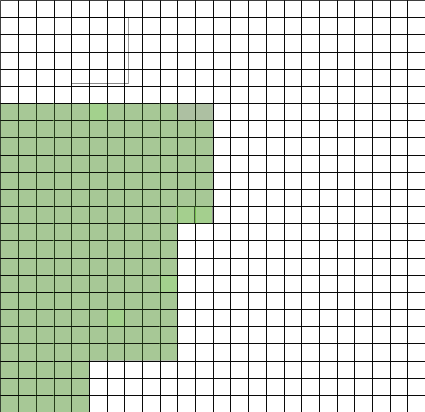
\includegraphics[width=.35\textwidth]{Pictures/DC/MC1.png}\caption{Marching cube}
	\end{figure}}
	\only<2>{
		\begin{figure}	
		\centering
		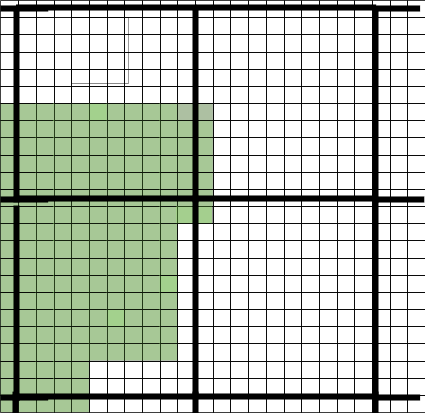
\includegraphics[width=.35\textwidth]{Pictures/DC/MC2.png}\caption{Marching cube}
		\end{figure}}
	\only<3>{
		\begin{figure}	
		\centering
		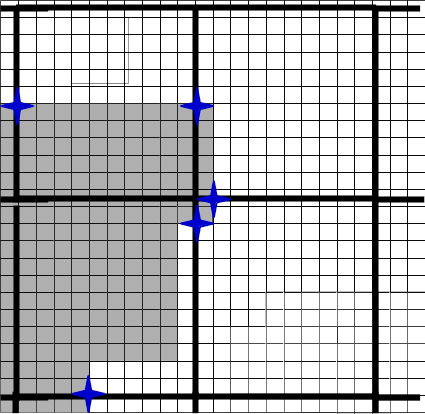
\includegraphics[width=.35\textwidth]{Pictures/DC/MC3.png}\caption{Marching cube}
		\end{figure}}
			\only<4>{
				\begin{figure}	
				\centering
				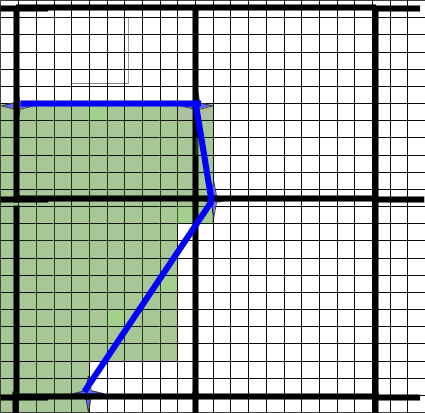
\includegraphics[width=.35\textwidth]{Pictures/DC/MC4.png}\caption{Marching cube}
	\end{figure}}
	\end{minipage}
	\begin{minipage}{0.49\textwidth}
	\only<1>{
	\begin{figure}	
	\centering
	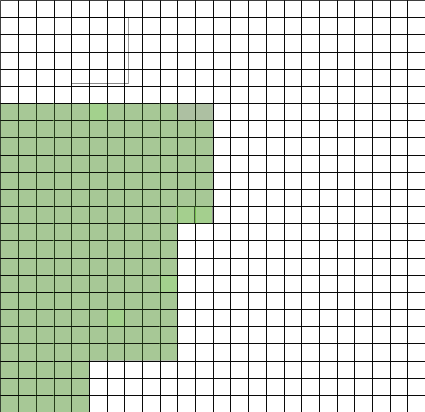
\includegraphics[width=.35\textwidth]{Pictures/DC/MC1.png}\caption{Dual Contouring}
	\end{figure}}
	\only<2>{
		\begin{figure}	
		\centering
		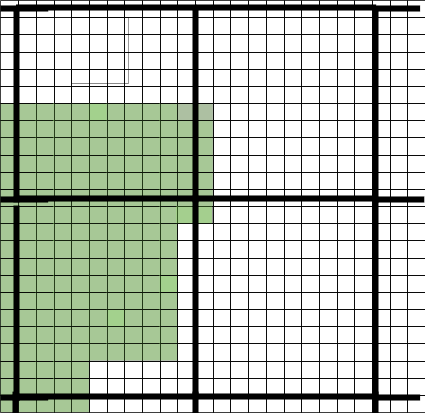
\includegraphics[width=.35\textwidth]{Pictures/DC/MC2.png}\caption{Dual Contouring}
		\end{figure}}
	\only<3>{
		\begin{figure}	
		\centering
		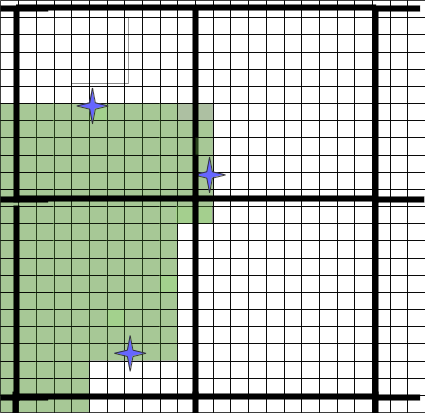
\includegraphics[width=.35\textwidth]{Pictures/DC/DC3.png}\caption{Dual Contouring}
		\end{figure}}
			\only<4>{
				\begin{figure}	
				\centering
				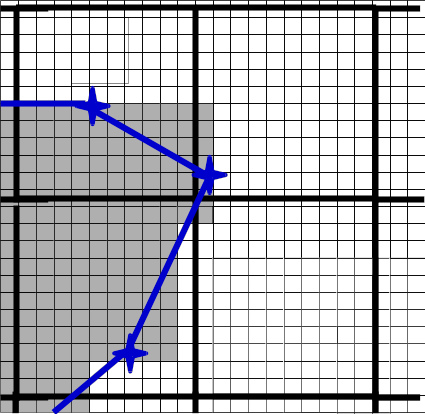
\includegraphics[width=.35\textwidth]{Pictures/DC/DC4.png}\caption{Dual Contouring}
	\end{figure}}
	
	\end{minipage}
%	\caption{Comparision of MC and DC for identical datasets. The vertices are created on the edges of the cubes for MC  and inside the cubes for DC. Please note that the sharp feature in the top right cube can only be reconstructed by DC. Figure from %\cite{FromVoxelsToPolygons}.
\end{frame}


\begin{frame}
	\frametitle{Dual Contouring}
	T
	\begin{overlayarea}{\textwidth}{.25 \textheight}
	Dual contouring on two different scales:
	\begin{itemize}
	\item Coarse scale: \\
	 Output: Closed surface made out of \textit{quads}; Parameter space
	\only<2>{\item Fine scale: \\
	Output: Vertices to fit for reconstructed geometry}
	\end{itemize}	
	\end{overlayarea}
	
	\begin{overlayarea}{\textwidth}{.75 \textheight}
	
	\begin{figure}
	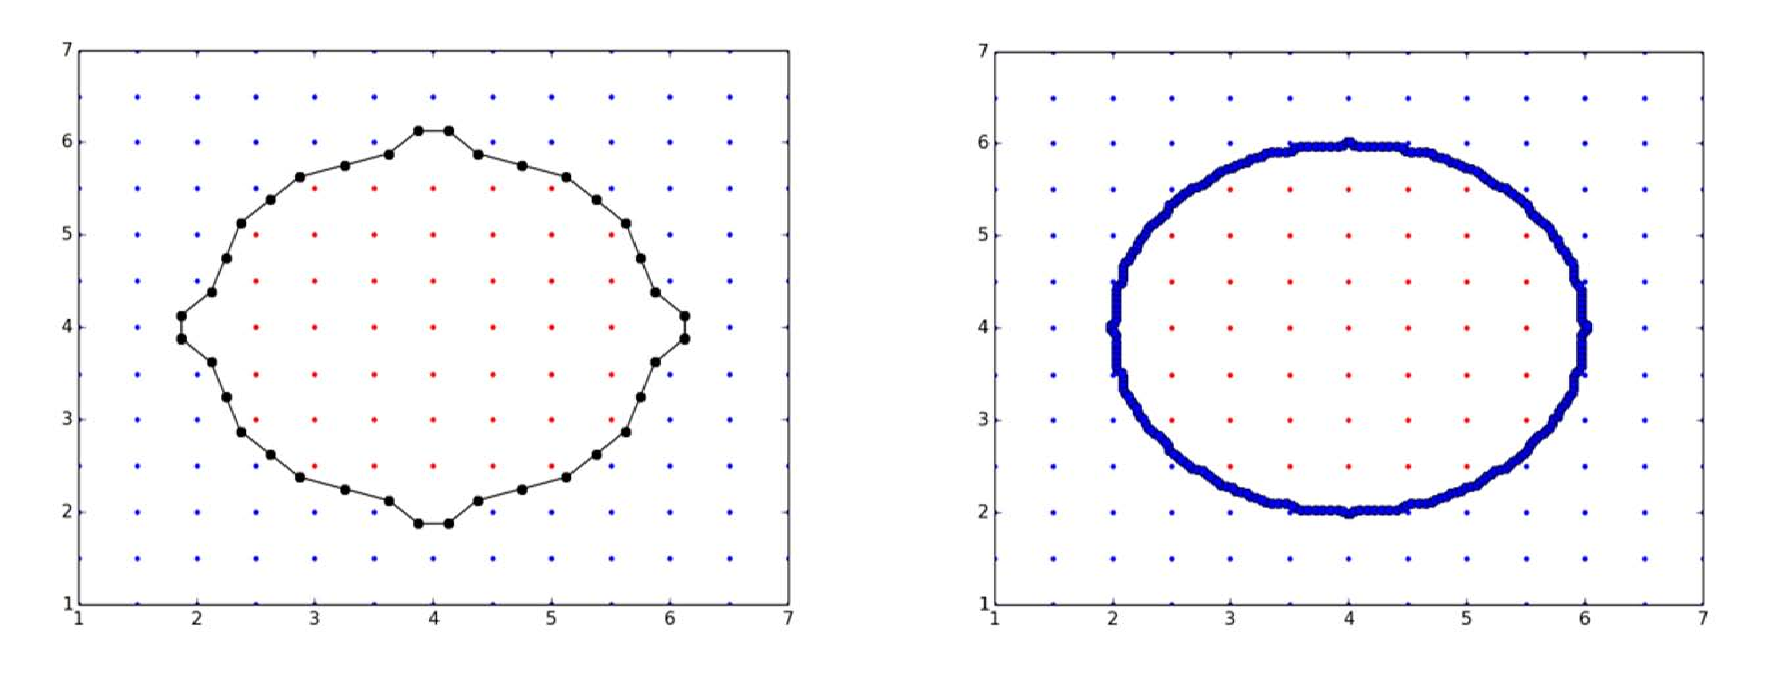
\includegraphics[scale=0.35]{Pictures/DC/DC_1.pdf}
	\end{figure}
	
	
%	\only<2>{
%	\begin{figure}
%	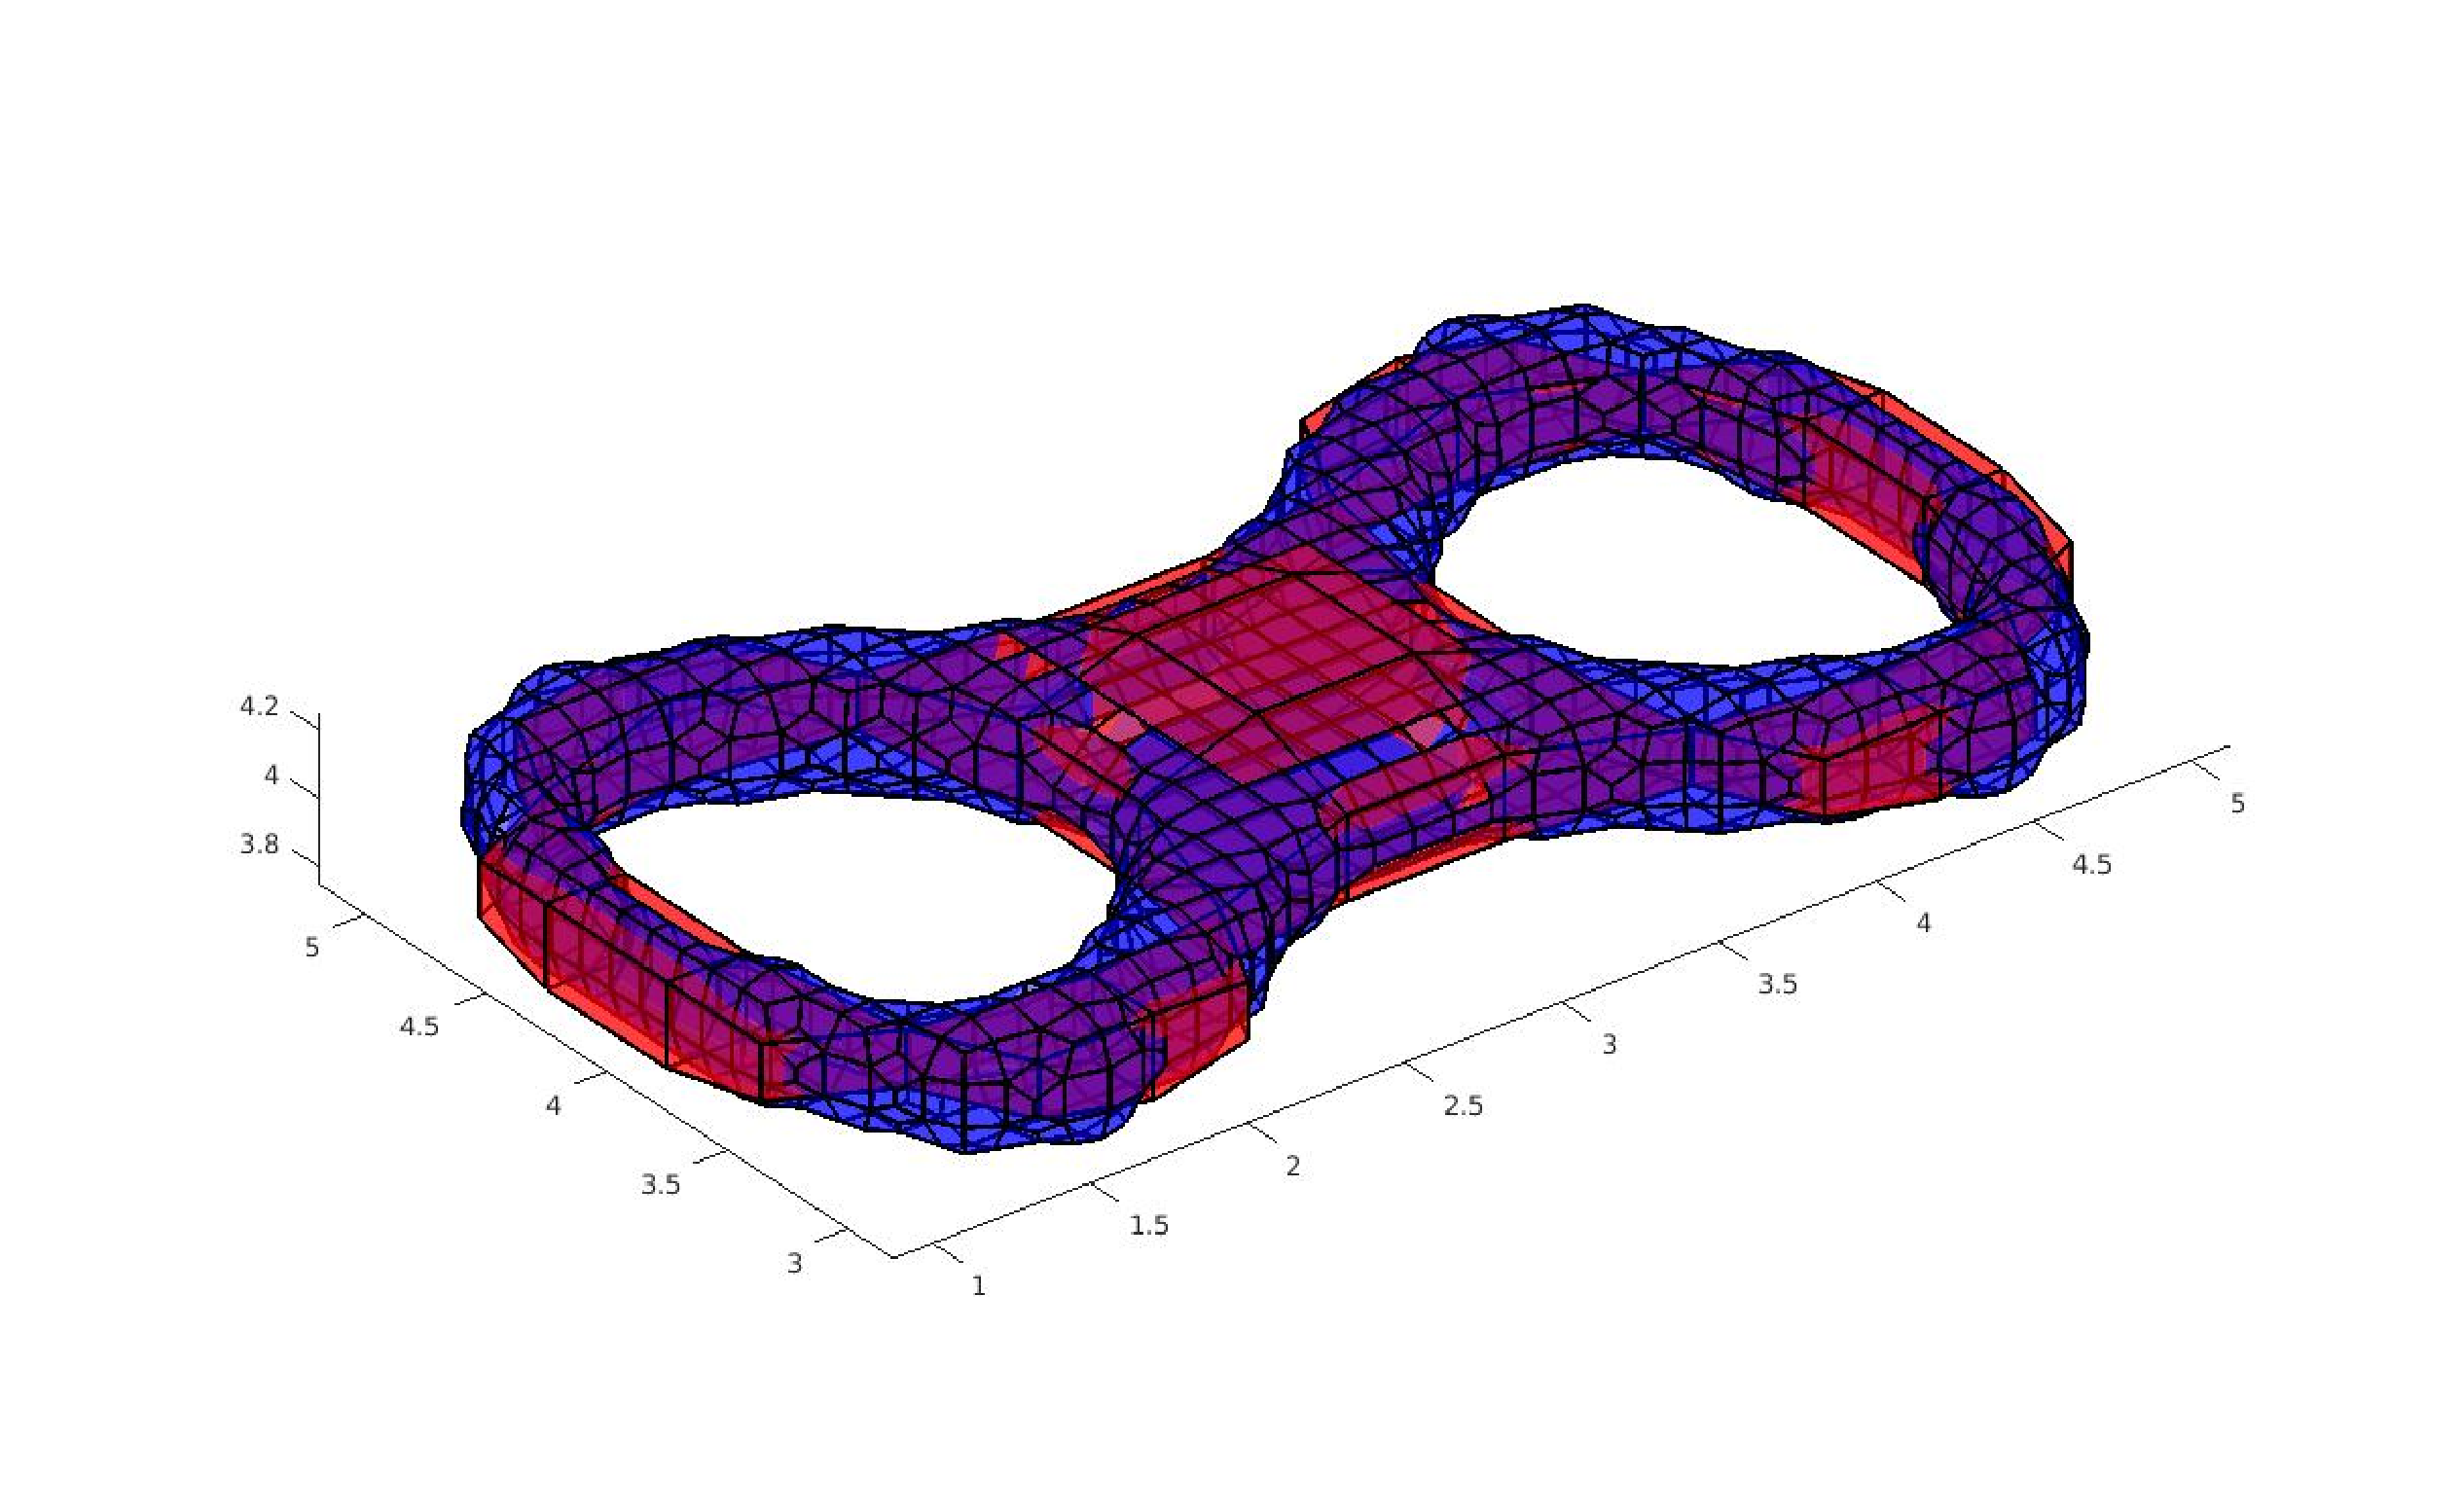
\includegraphics[scale=0.2]{Pictures/DC/doubleTorus.pdf}
%	\end{figure}
%	}
	\end{overlayarea}
	
\end{frame}



\subsection{Projection and Parametrization}

\begin{frame}

	\frametitle{Projection and Parametrization}
	
	\begin{itemize}
	\item Points from finer grid are projected to quads of the coarser grid 
	\item Parameters \textit{u} and \textit{v} are found for each quad
	\item This information is needed for the algorithms in the last part of the pipeline
	\end{itemize}
	\begin{figure}
	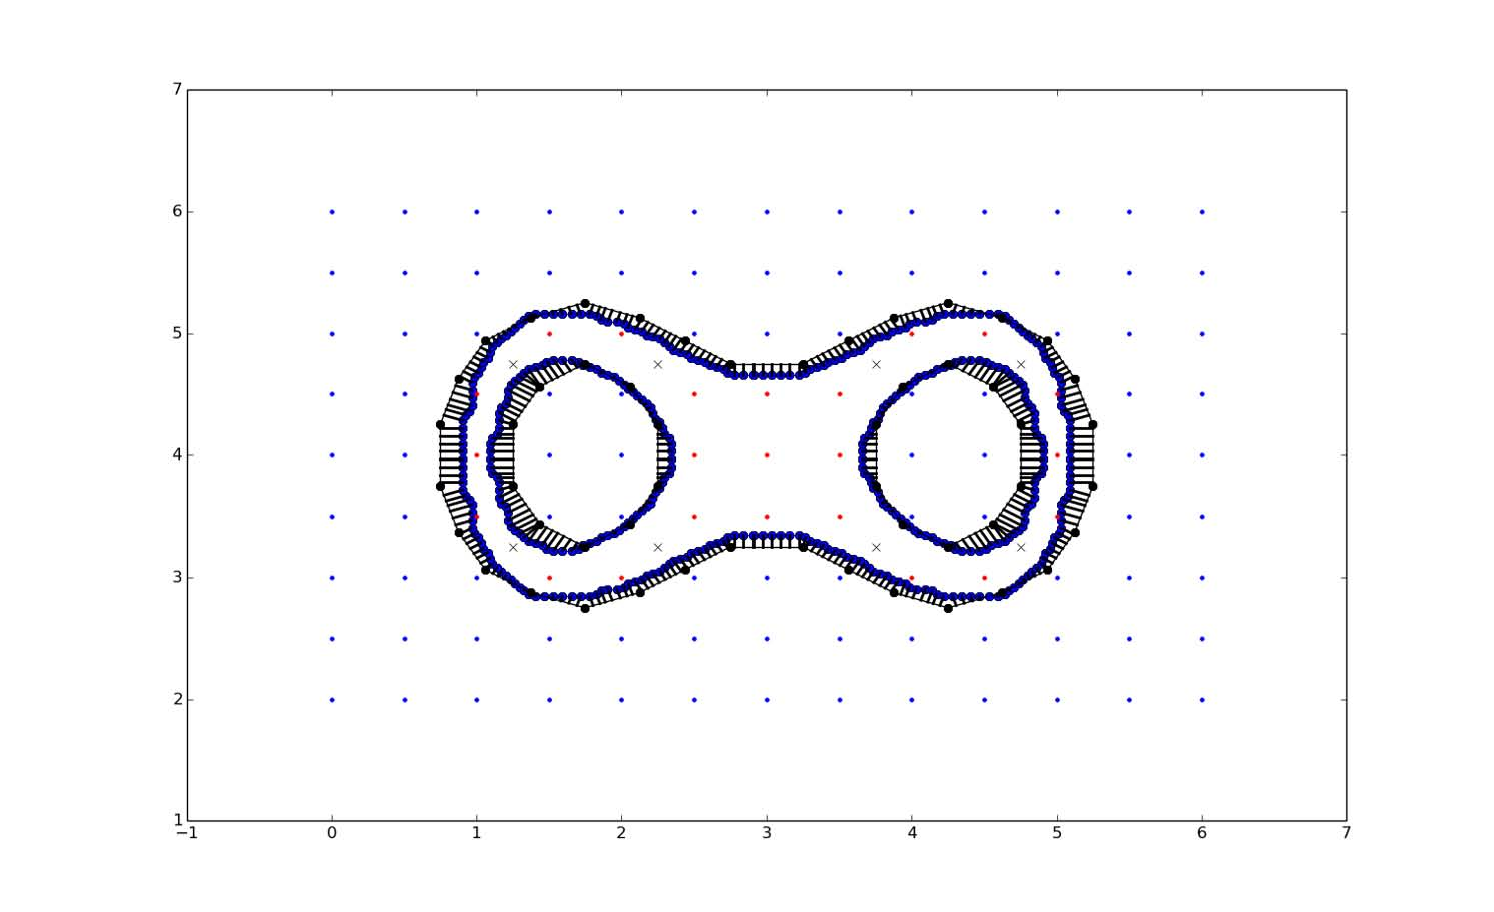
\includegraphics[scale=0.35]{Pictures/DC/DC_2.pdf}
	\end{figure}
	
\end{frame}





